% =========================================================
% 8. CROSS-CUTTING CONCEPTS
% =========================================================
\section{Cross-cutting Concepts}

\minititle{Content}
This section describes crosscutting concepts (practices, patterns, regulations or solution ideas). Such concepts are often related to multiple building blocks. They may include many different topics, such as the topics shown in the following diagram:

% Figure 3:
\begin{figure}[H]
  \centering
  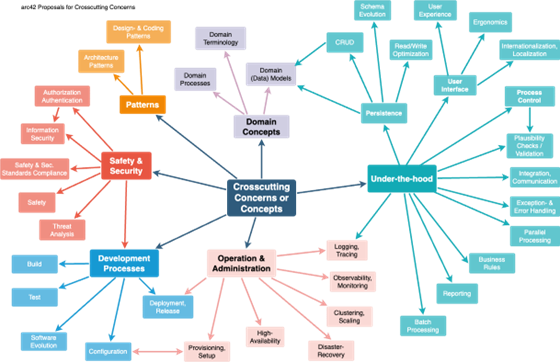
\includegraphics[width=0.85\textwidth]{cross-cutting-concerns.png}
  \caption{Chaotic Cross-Cutting Concerns in arc42, Domain Concepts etc. belong into a DDD subchapter, Safety, Security, under-the hood are quality categories in ISO 25010 (clean this up for your project).}
  \label{fig:ccc}
\end{figure}

% Additional course comment:
% Carefully think if your planned content here does not better belong into the other chapters!!!
% Development issues can be discussed here, but deployment belongs to the operational model.
% Similarly, most of the under-the-hood entries either belong into the ADM,
% or the quality discussion, or process model analysis and modeling.

\minititle{Motivation}
Concepts form the basis for conceptual integrity (consistency, homogeneity) of the architecture. Thus, they are an important contribution to achieve inner qualities of your system.

This is the place in the template that we provided for a cohesive specification of such concepts.

Many of these concepts relate to or influence several of your building blocks.

\minititle{Form}
The form can be varied:
\begin{itemize}
  \item concept papers with any kind of structure
  \item example implementations, especially for technical concepts
  \item cross-cutting model excerpts or scenarios using notations of the architecture views
\end{itemize}

\minititle{Structure}
Pick only the most-needed topics for your system and assign each a level-2 heading in this section (e.g. 8.1, 8.2 etc).

DO NOT ATTEMPT to cover all of the topics of the aforementioned diagram.

\minititle{Further Information}
See Concepts in the arc42 documentation:
\href{https://docs.arc42.org/section-8/}{https://docs.arc42.org/section-8/}

\subsection{\textless Concept 1\textgreater}
\textless explanation\textgreater

\subsection{\textless Concept 2\textgreater}
\textless explanation\textgreater

\subsection{\textless Concept n\textgreater}
\textless explanation\textgreater

